\documentclass[tikz,border=2pt,11pt]{standalone}
\usetikzlibrary{arrows.meta}
\usetikzlibrary{decorations.pathreplacing}
\usetikzlibrary{calc}
\usetikzlibrary{positioning}
\usepackage{amsmath}
\usepackage{amssymb}
\usepackage{xcolor}
\usepackage{tikz}
\newcommand{\RR}{\mathbb R}
\newcommand{\CC}{\mathbb C}
\newcommand{\ii}{\mathrm i}
\newcommand{\EE}{\mathcal E}
\newcommand{\abs}[1]{\lvert #1\rvert}
\newcommand{\norm}[1]{\lVert #1\rVert}
\DeclareMathOperator{\re}{Re}
\begin{document}
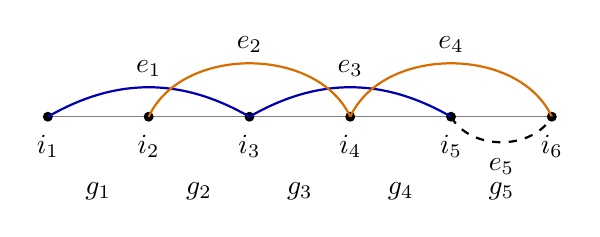
\begin{tikzpicture}[x=1.28cm,y=0.9cm,>=stealth,
  olda/.style={draw=blue!70!black,thick},
  oldb/.style={draw=orange!85!black,thick},
  added/.style={draw=black,thick,dashed}]
  \draw[gray] (0,0)--(5,0);
  \foreach \a in {1,...,6} {
    \fill (\a-1,0) circle (1.8pt);
    \node[below=3pt] at (\a-1,0) {$i_{\a}$};
  }
  \draw[olda] (0,0) to[bend left=30] node[above,pos=.5] {$e_1$} (2,0);
  \draw[olda] (2,0) to[bend left=30] node[above,pos=.5] {$e_3$} (4,0);
  \draw[oldb] (1,0) to[bend left=65] node[above,pos=.5] {$e_2$} (3,0);
  \draw[oldb] (3,0) to[bend left=65] node[above,pos=.5] {$e_4$} (5,0);
  \draw[added] (4,0) to[bend right=60] node[below=2pt,pos=.5] {$e_5$} (5,0);
  \foreach \a in {1,...,5} {
    \node at (\a-.5,-1.05) {$g_{\a}$};
  }
\end{tikzpicture}
\end{document}
